\documentclass[linenumbers]{aastex631}

\newcommand{\vdag}{(v)^\dagger}
\newcommand\aastex{AAS\TeX}
\newcommand\latex{La\TeX}
\newcommand{\Msun}{\mathrm{M_{\odot}}}
\newcommand{\Rsun}{\mathrm{R_{\odot}}}
\newcommand{\MWD}{M_{\mathrm{WD}}}
\newcommand{\Mstar}{M_{\star}}
\newcommand{\alphace}{\alpha_{\mathrm{CE}}}
\newcommand{\alphath}{\alpha_{\mathrm{th}}}
\newcommand{\alpharec}{\alpha_{\mathrm{rec}}}
\newcommand{\Ebind}{E_{\mathrm{bind}}}
\newcommand{\Egrav}{E_{\mathrm{grav}}}
\newcommand{\Eint}{E_{\mathrm{int}}}
\newcommand{\Eth}{E_{\mathrm{th}}}
\newcommand{\Erec}{E_{\mathrm{rec}}}
\newcommand{\Porb}{P_{\mathrm{orb}}}
\newcommand{\au}{\, \mathrm{au}}


\begin{document}

\title{Wide Post-Mass Transfer White Dwarf Binaries}

%\author[0000-0002-0786-7307]{Greg J. Schwarz}
%\affiliation{American Astronomical Society \\
%1667 K Street NW, Suite 800 \\
%Washington, DC 20006, USA}

\author{Runqiu Ye}
\affiliation{Carnegie Mellon University}

%\collaboration{20}{(AAS Journals Data Editors)}
%
%\author{F.X Timmes}
%\affiliation{Arizona State University}
%\affiliation{AAS Journals Associate Editor-in-Chief}
%
%\author{Amy Hendrickson}
%\altaffiliation{AASTeX v6+ programmer}
%\affiliation{TeXnology Inc.}
%
%\author{Julie Steffen}
%\affiliation{AAS Director of Publishing}
%\affiliation{American Astronomical Society \\
%1667 K Street NW, Suite 800 \\
%Washington, DC 20006, USA}

\begin{abstract}

(***TO-DO***) This example manuscript is intended to serve as a tutorial and template for
authors to use when writing their own AAS Journal articles. The manuscript
includes a history of \aastex\ and includes figure and table examples to illustrate these features. Information on features not explicitly mentioned in the article can be viewed in the manuscript comments or more extensive online
documentation. Authors are welcome replace the text, tables, figures, and
bibliography with their own and submit the resulting manuscript to the AAS
Journals peer review system.  The first lesson in the tutorial is to remind
authors that the AAS Journals, the Astrophysical Journal (ApJ), the
Astrophysical Journal Letters (ApJL), the Astronomical Journal (AJ), and
the Planetary Science Journal (PSJ) all have a 250 word limit for the 
abstract\footnote{Abstracts for Research Notes of the American Astronomical 
Society (RNAAS) are limited to 150 words}.  If you exceed this length the
Editorial office will ask you to shorten it. This abstract has 161 words.

\end{abstract}


\keywords{(***TO-DO***) Classical Novae (251) --- Ultraviolet astronomy(1736) --- History of astronomy(1868) --- Interdisciplinary astronomy(804)}

\section{Introduction} \label{sec:intro}

Common envelope (CE) is the outcome of unstable mass transfer. During CE, both stars orbit inside an envelope and spiral inward. If the energy liberated in this process is enough to eject the CE, then the result of CE process is a close binary. If, on the contrary, the liberated energy is not enough to eject the envelope, then the result of the process is a merger. In observation results, a number of WD+MS binaries are wider than expected, and CE is expected to be the main channel to form these white dwarf binaries \cite{yamaguchi_hi, yamaguchi_lo}. In the MESA model utilized by \cite{yamaguchi_hi, yamaguchi_lo}, wide post-CE WD+MS binaries can be formed in a certain range of initial separation with only gravitational and internal energy included in the calculation. 

In this paper, we are going to explore the formation of these wide post-mass transfer WD+MS binaries with COSMIC model. We perform COSMIC simulation on both individual binary star systems and sampled population to explore the formation of WD+MS binaries under different conditions. In section \ref{sec:ce}, we are going to investigate formation of individual wide WD+MS binaries through CE for a variety of variables, including initial mass, initial separation, CE efficiency, and the energy budget of the CE. In section \ref{sec:stable}, we are going to explore the formation of individual wide WD+MS binaries through stable mass transfer. In section \ref{sec:population}, we will research on how different COSMIC model affect simulation results of a sample population of binary star systems, and how the formation of post WD+MS binaries depends on various parameters.

\section{Common Envelope} \label{sec:ce}
In \cite{yamaguchi_hi, yamaguchi_lo}, the author discussed the formation of WD+MS binaries through CE for both high-mass and low-mass systems, and it was found that wide WD+MS systems can be formed for certain energy budgets and certain initial separation in the MESA model. We hope to explore similar models in COSMIC.

In \cite{yamaguchi_hi, yamaguchi_lo}, to explore the dependency of the final separation $a_f$ in the post-CE binary on the initial separation $a_i$ in the pre-MT binary, the author first run a stellar evolution model of the primary star using MESA. Its evolution up to AGB phase is followed. With the model, the binding energy of the CE is calculated as

\begin{equation}
	E_{\mathrm{bind}} = E_{\mathrm{grav}} + E_{\mathrm{int}} = \int_{M_{\mathrm{core}}}^{M_{\mathrm{tot}}} -\frac{Gm}{r(m)} + U(m) dm,
	\label{budget-int}
\end{equation}
or
\begin{equation}
	E_{\mathrm{bind}} = E_{\mathrm{grav}} + \alphath E_{\mathrm{th}} + \alpharec E_{\mathrm{rec}}.
	\label{budget-th-rec}
\end{equation}
After that, the change of separation through CE evolution is calculated using
\begin{equation}
	E_{\mathrm{bind}} = \alphace \left(-\frac{G\MWD \Mstar}{2a_f}+\frac{GM_i \Mstar}{2a_i}\right).
	\label{ebind-sep}
\end{equation}

In COSMIC, the CE is modeled using a structural parameter $\lambda$, where
\begin{equation}
	\Ebind = \frac{G M_i M_{\mathrm{env}}}{\lambda R_i}.   
	\label{ebind}
\end{equation}
This $\lambda$ is represented in COSMIC as the \verb|lambdaf| flag in \verb|BSEDict|. To compare MESA model with COSMIC, we intend to compare how the energy budget utilized by \cite{yamaguchi_hi, yamaguchi_lo} matches with the CE model in COSMIC. We approach this by calculating the effective $\lambda$ value for each of the energy budget used in \cite{yamaguchi_hi, yamaguchi_lo}. 

\subsection{High Mass Systems $(7 \Msun + 1 \Msun)$} \label{subsec:high}

\subsubsection{Methods and results}

In \cite{yamaguchi_hi}, the lower limit of WD mass $M_{\mathrm{MD, min}}$ in the observational sample is calculated to be $1.244\Msun \sim 1.418\Msun$. The corresponding mass of MS progenitor is expected to be in the range of $6 \sim 9 \Msun$, and the companion mass has median around $1\Msun$. MESA results for $7\Msun + 1\Msun$ systems is documented in \cite{yamaguchi_hi}. Hence, we also consider a $7\Msun + 1\Msun$ evolution model in COSMIC and compare the results with those in \cite{yamaguchi_hi}.

We run COSMIC binary evolution simulation of a $7\Msun + 1\Msun$ system and investigate how the final separation $a_f$ depends on the initial separation $a_i$ and the CE parameter $\lambda$. We vary the initial separation in range $2 \sim 8 \au$ with $400$ steps. We vary the CE flag \verb|lambdaf| in range $0 \sim -100$, which corresponds to $\lambda = 0 \sim 100$, with $2000$ steps. Also, we run these parameters with four different CE efficiencies — $\alphace = 1$, $\alphace = 0.9$, $\alphace = 0.6$, and $\alphace = 0.3$, the same as documented in \cite{yamaguchi_hi}. In total, for $4$ different CE efficiency $\alphace$, we run a grid of $80000$ binary star systems with different initial separation $a_i$ and CE parameter $\lambda$.

After simulation is finished, we select the time-step when the system finished CE for the first time (\verb|evol_type = 8|). At this moment, if the system is a WD+MS system, we record their separation as the final separation $a_f$. Otherwise, we set $a_f = 0$ and consider this initial condition unable to produce a WD+MS system.

We create four heat maps for the four different CE efficiencies. In Figure \ref{res_hi}, we plot the final separation $a_f$ of the WD+MS systems against initial separation $a_i$ and the CE flag \verb|lambdaf|$= - \lambda$.

\begin{figure}
	\centering
	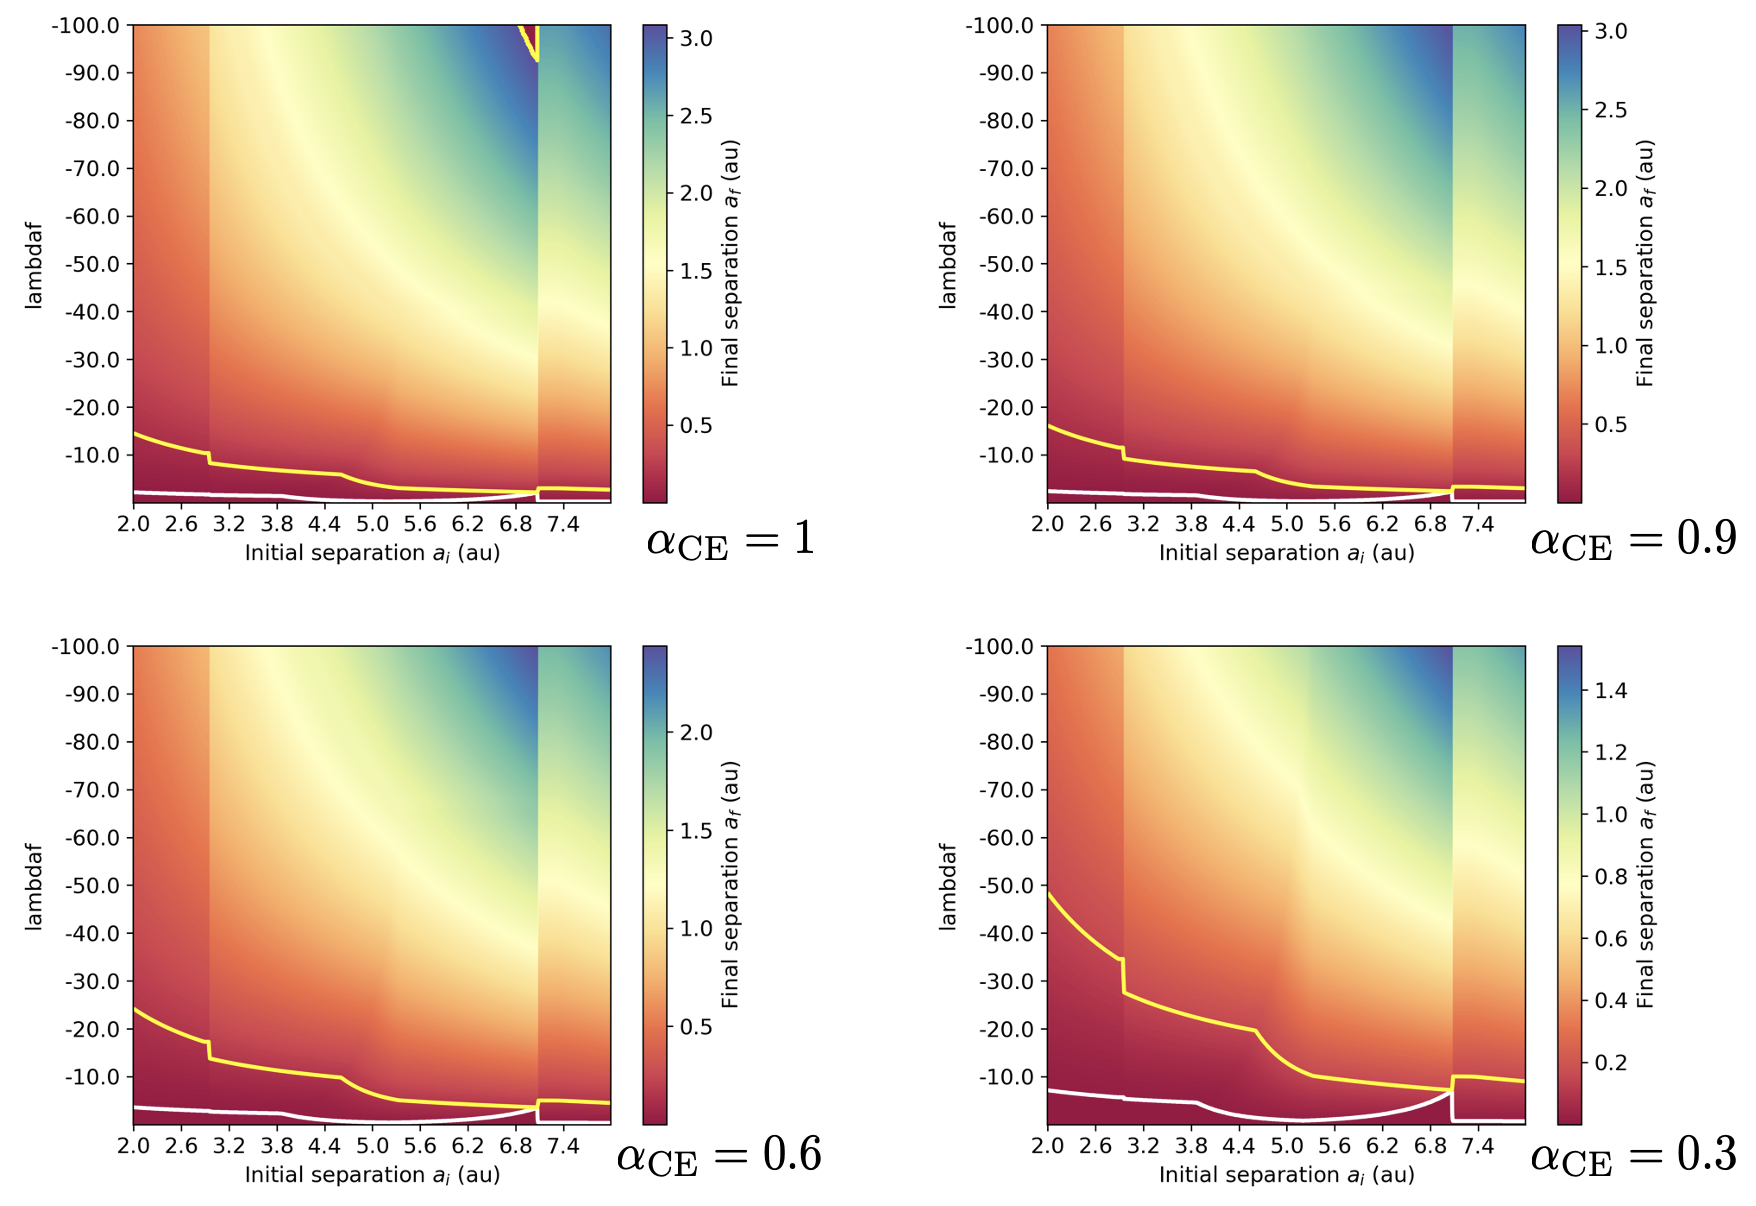
\includegraphics[width=0.8\linewidth]{7+1results.png}
	\caption{ Heat map of final separation $a_f$ against initial separation $a_i$ and CE flag lambdaf$=-\lambda$. Different panels represent four different CE efficiencies $\alphace = 1$, $0.9$, $0.6$, and $0.3$. The white and yellow contour corresponds to $a_f = 0.01 \au$ and $a_f = 0.15 \au$ respectively. WD+MS binaries is not possible for separation smaller than $0.01 \au$, and $0.15 \au$ is the minimum separation of wide WD+MS binaries in observational results. Outside the white contour no desired system forms.}
	\label{res_hi}
\end{figure}

\subsubsection{Discussions}

There are several interesting points of the results. First of all, as $\alphace$ decreases, the final separation decreases in general. This can be explained by Equation \ref{ebind-sep}. Qualitatively, note that more energy from the orbit is needed to eject the envelope for low $\alphace$, so the resulting $a_f$ is expected to be smaller. 

It is worth noting that most of these systems experience two mass transfer phases in COSMIC before reaching WD+MS. That is, during the evolution process, two CE processes take place, between which there is a period of time. By checking the \verb|bpp| array, which documents the evolution processes of the binary star systems, we found that (***TO-DO***) fraction of all our simulated binaries experience two CE processes before reaching WD+MS. When the primary loses too much mass during the first CE, the CE process ends. After the primary fills its Roche lobe and has a large enough envelope again, the CE process resumes and causes two CE processes in total.

From Figure \ref{res_hi}, we also notice that the final separation $a_f$ jumps obviously at about $2.9 \au$, and $7.1 \au$. After investigating the \verb|bpp| array of these simulations, we find out the jump at about $2.9 \au$ and $7.1 \au$ is likely due to the difference of \verb|kstar_1| at the start of RLOF. For $a_i < 2.9 \au$, RLOF starts when the primary is on the giant branch (GB) with \verb|kstar_1 3|. For $a_i = 2.9 \au$, RLOF starts when the primary is experiencing core Helium burning (CHeB) with \verb|kstar_1 = 4|. For $2.9 \au < a_i < 7.1 \au$, RLOF starts when the primary is on E-AGB with \verb|kstar_1 = 5|. For $a_i > 7.1 \au$, RLOF starts when the primary is on TP-AGB with \verb|kstar_1 = 6|. For different star type, the structure and mass of the envelope is different, leading to different binding energy $\Ebind$ and thus different final separation $a_f$.

\begin{figure}
	\centering
	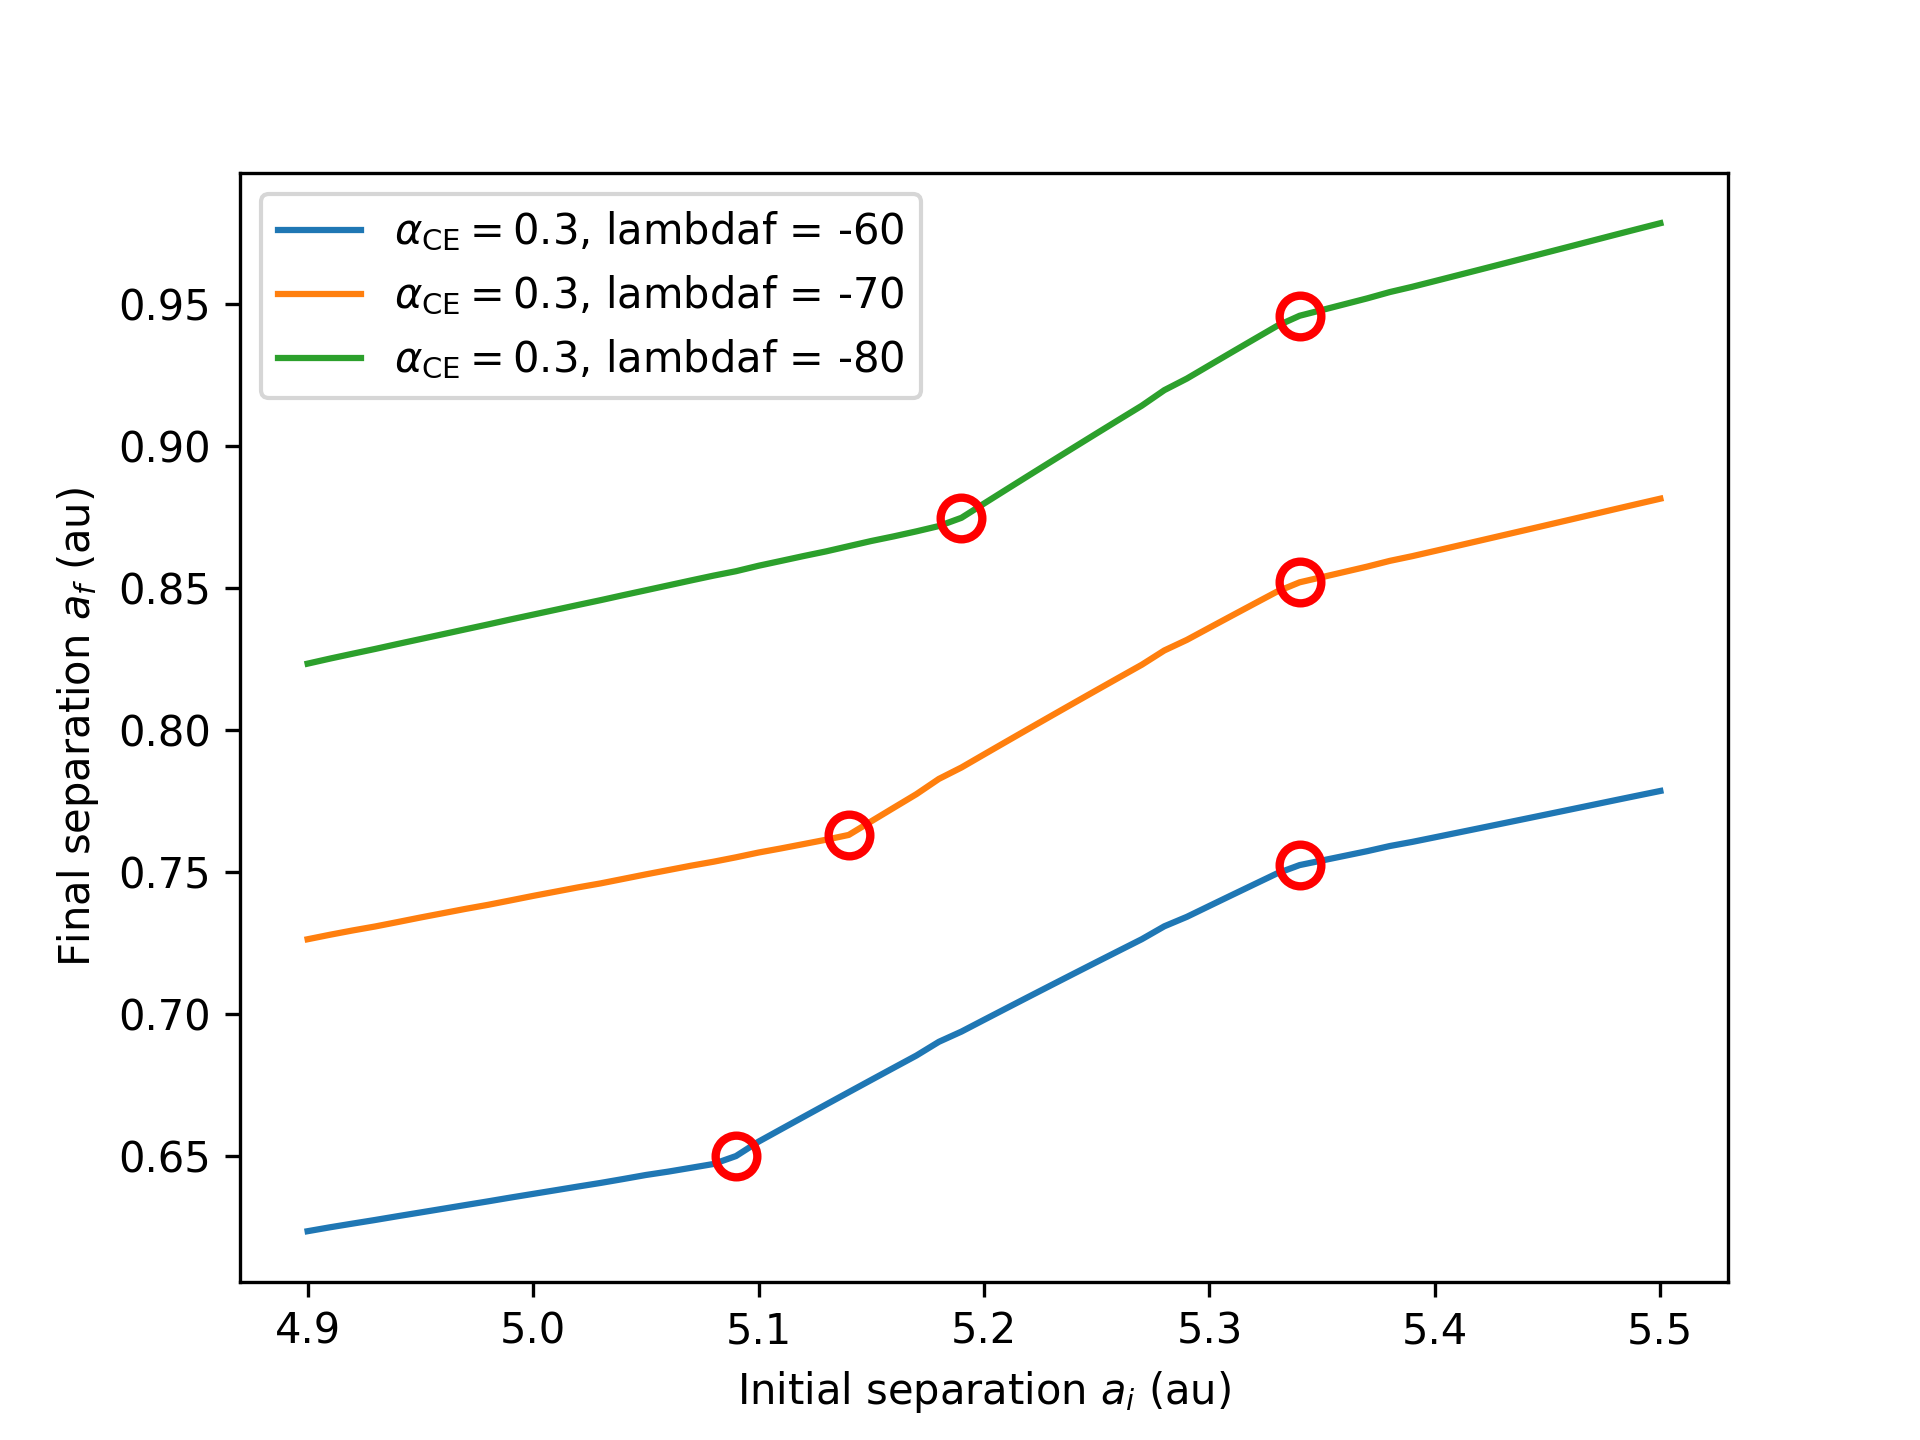
\includegraphics[width = 0.5\linewidth]{jump-zoom.png}
	\caption{Dependence of final separation $a_f$ on initial separation $a_i$ for $\alphace = 0.3$. Simulation results of $\lambda_f = 60$, $70$, and $80$ are shown. The red circles emphasizes the jump of final separation as initial separation increases.}
	\label{jump-zoom}
\end{figure}

Inspecting more closely, we find that the final separation $a_f$ jumps at about $5.2 \sim 5.4 \au$. This is especially obvious with $\alphace = 0.3$. To illustrate, we zoom in the simulation results of $\alphace = 0.3$, and present the change of final separation $a_f$ as initial separation $a_i$ increases in Figure \ref{jump-zoom}. From here, we can clearly see two jumps — one between $5.1\au$ and $5.2\au$, the other at $5.34\au$. To explain this, we again go to the \verb|bpp| array of these systems. We notice that the first jump is probably because the evolution process changes from \textbf{3-7-8-4-3-7-8-4} to \textbf{3-7-8-7-8-4}. This means that for relatively larger initial separation $a_i$, the primary fills its Roche lobe all the time, leading to more mass loss during a shorter timescale and thus larger final separation. Also, the second jump is probably because \verb|kstar_1| changes from \verb|8| (Naked Helium Star Hertzsprung Gap) to \verb|9| (Naked Helium Star Giant Branch) at the start of the second common envelope. This changes the binding energy of the common envelope and thus changes the final separation.

Finally, notice that there exists a small triangular gap in the figure for $\alphace = 1$. This is because \verb|kstar_1| becomes a neutron star and no rows in the \verb|bpp| gets selected.

In conclusion, with a large \verb|lambdaf|, it is possible to create wide post-mass transfer WD+MS systems with final separation $a_f > 0.15 \au$, which is the minimal separation of our observed objects. In next section, we will compare these results with default settings in COSMIC and with results in \cite{yamaguchi_hi}, in order to investigate the possibility of forming wide WD+MS systems through CE.

\subsubsection{Comparison}
After we have obtained the simulation results for different initial conditions, now we can calculate the effective $\lambda$ that matches with results in \cite{yamaguchi_hi}. For each fixed initial separation $a_i$, we loop through the COSMIC results with the same initial separation, and find the \verb|lambdaf| value that results in a final separation closest to MESA model results. We record this \verb|lambdaf| as the effective $\lambda$ that matches the binding energy formalism at initial separation $a_i$.

\begin{figure}
	\centering
	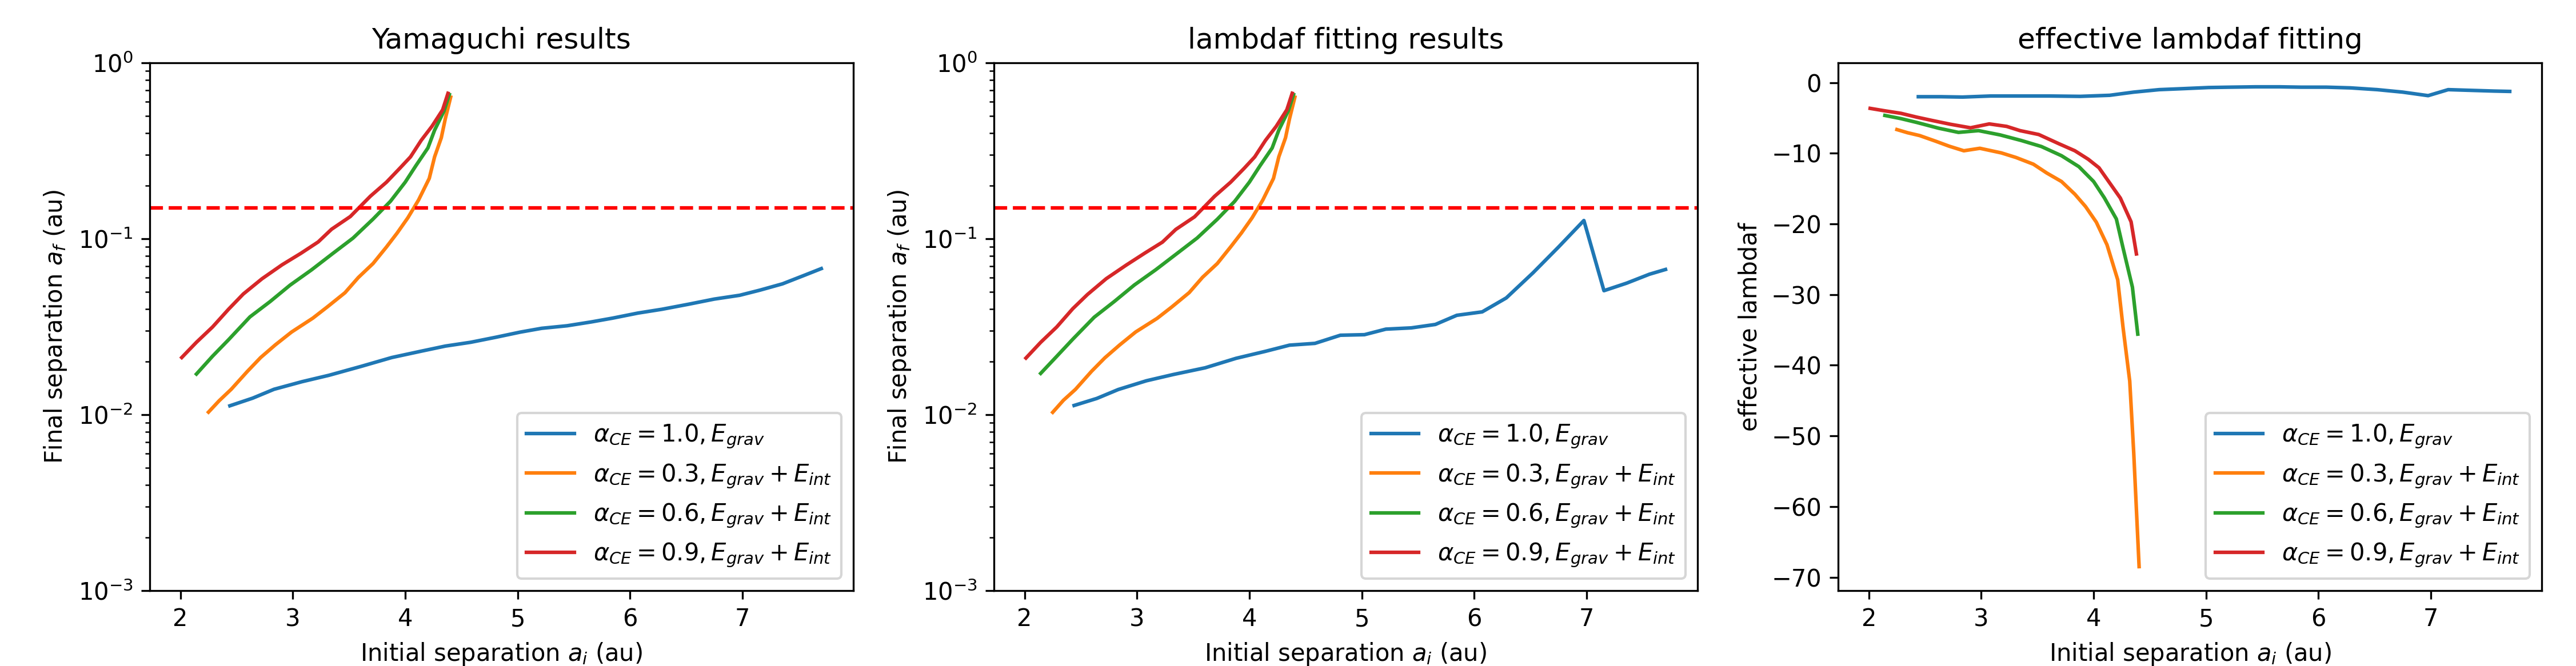
\includegraphics[width=0.9\linewidth]{7+1fit.png}
	\caption{Effective $\lambda$ fitting results of a $7\Msun + 1\Msun$ system for common envelope structure in MESA. Left panel: MESA results in \cite{yamaguchi_hi} of how final separation $a_f$ depends on initial separation $a_i$. Central panel: COSMIC results of how final separation $a_f$ depends on initial separation $a_i$, produced by the effective $\lambda$ calculated. Right panel: effective $\lambda$ in COSMIC that corresponds to the MESA results for each initial separation $a_i$. The red dashed line in the left and middle panel represents $0.15 \au$, which is the minimal separation for observed wide post-CE WD+MS binaries.}
	\label{fit_hi}
\end{figure}

We present the fitting results for energy budget $\Ebind = \Egrav + \Eint$ in Figure \ref{fit_hi}. Notice that in the central panel, there is a small bump of the blue line. This is because at $6 \sim 7 \au$, we cannot reach such low final separation in COSMIC while forming a WD+MS binary at the same time. From the left panel, we can see that it is possible to create WD+MS binaries with final separation $>0.15 \au$ in MESA as long as internal energy $\Eint$ is included. However, in the right panel we show that this correspond to very large \verb|lambdaf| in COSMIC ($\lambda > \sim 20$).

\begin{figure}
	\centering
	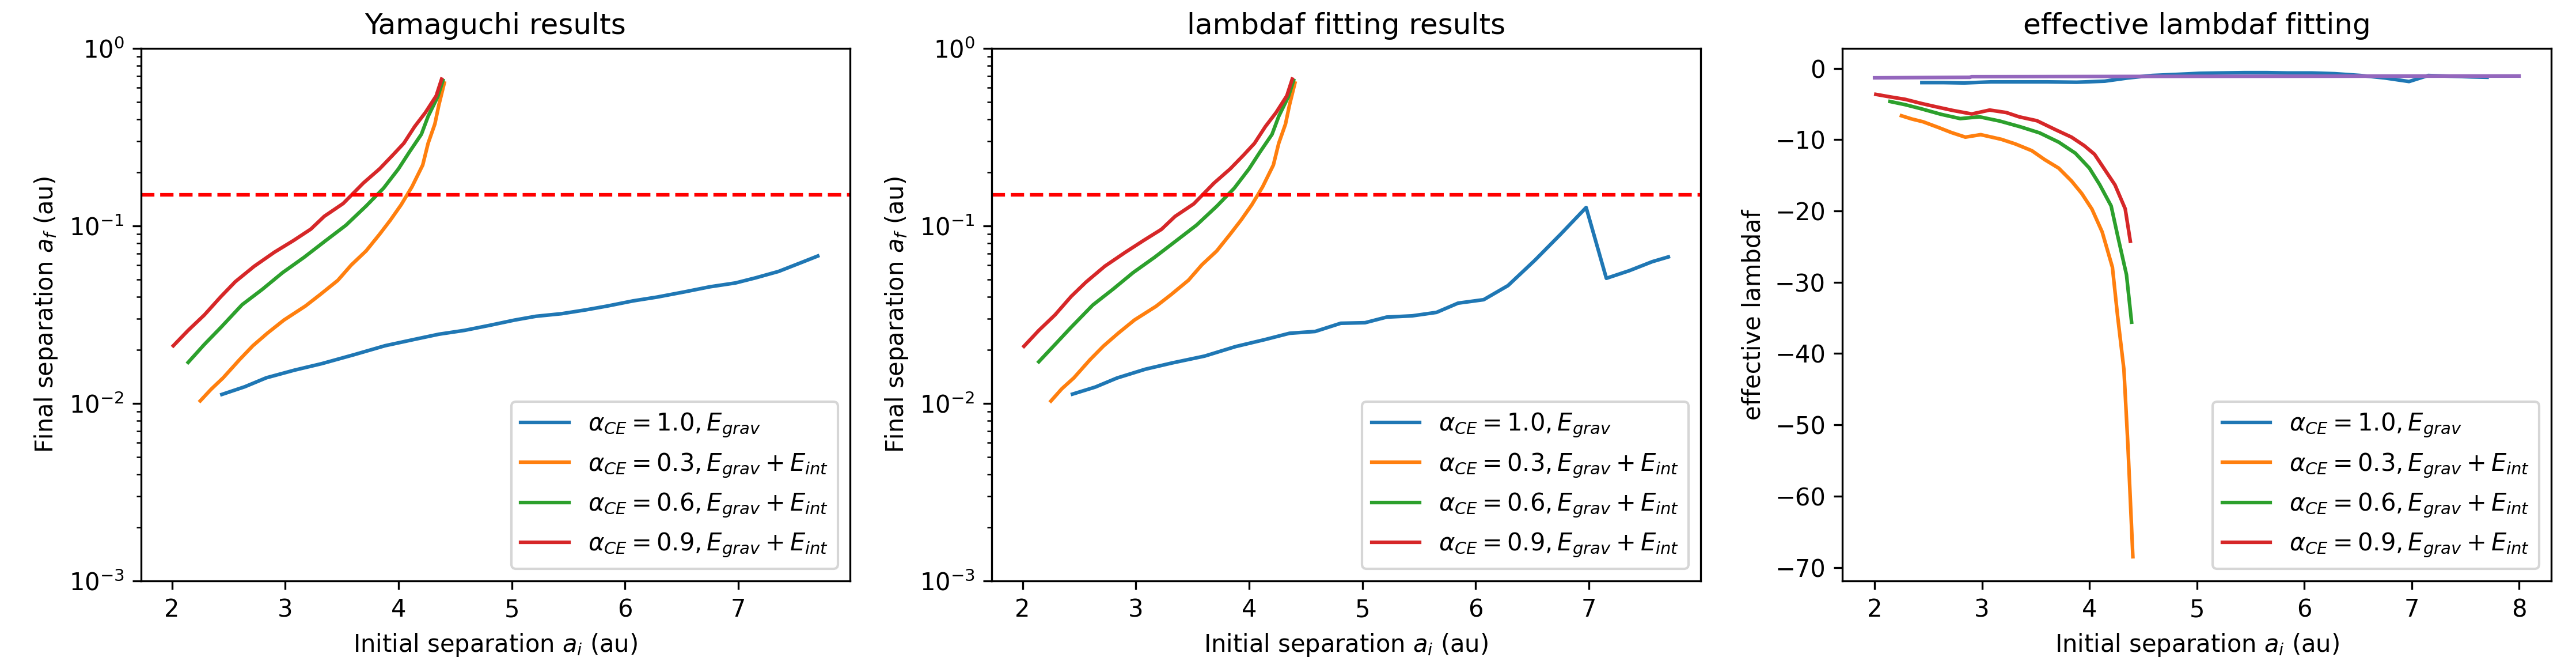
\includegraphics[width=0.9\linewidth]{7+1cmp.png}
	\caption{Same as Figure \ref{fit_hi}, but with default $\lambda$ in COSMIC model included in the right panel.}
	\label{fit_cmp_hi}
\end{figure}

To further compare with the default $\lambda$ value in COSMIC, we include in the right panel an extra line which represents the default $\lambda$ value in COSMIC. This default $\lambda$ in the COSMIC model is calculated following Appendix A of \cite{claeys2014theoretical}. For all of our case, we have $M_{\mathrm{env}} > 1$. The results is shown in Figure \ref{fit_cmp_hi}. Notice that the default $\lambda$ value is at order $\sim 1$, far smaller than the effective $\lambda$ needed to recreate results in \cite{yamaguchi_hi}.

\begin{figure}
	\centering
	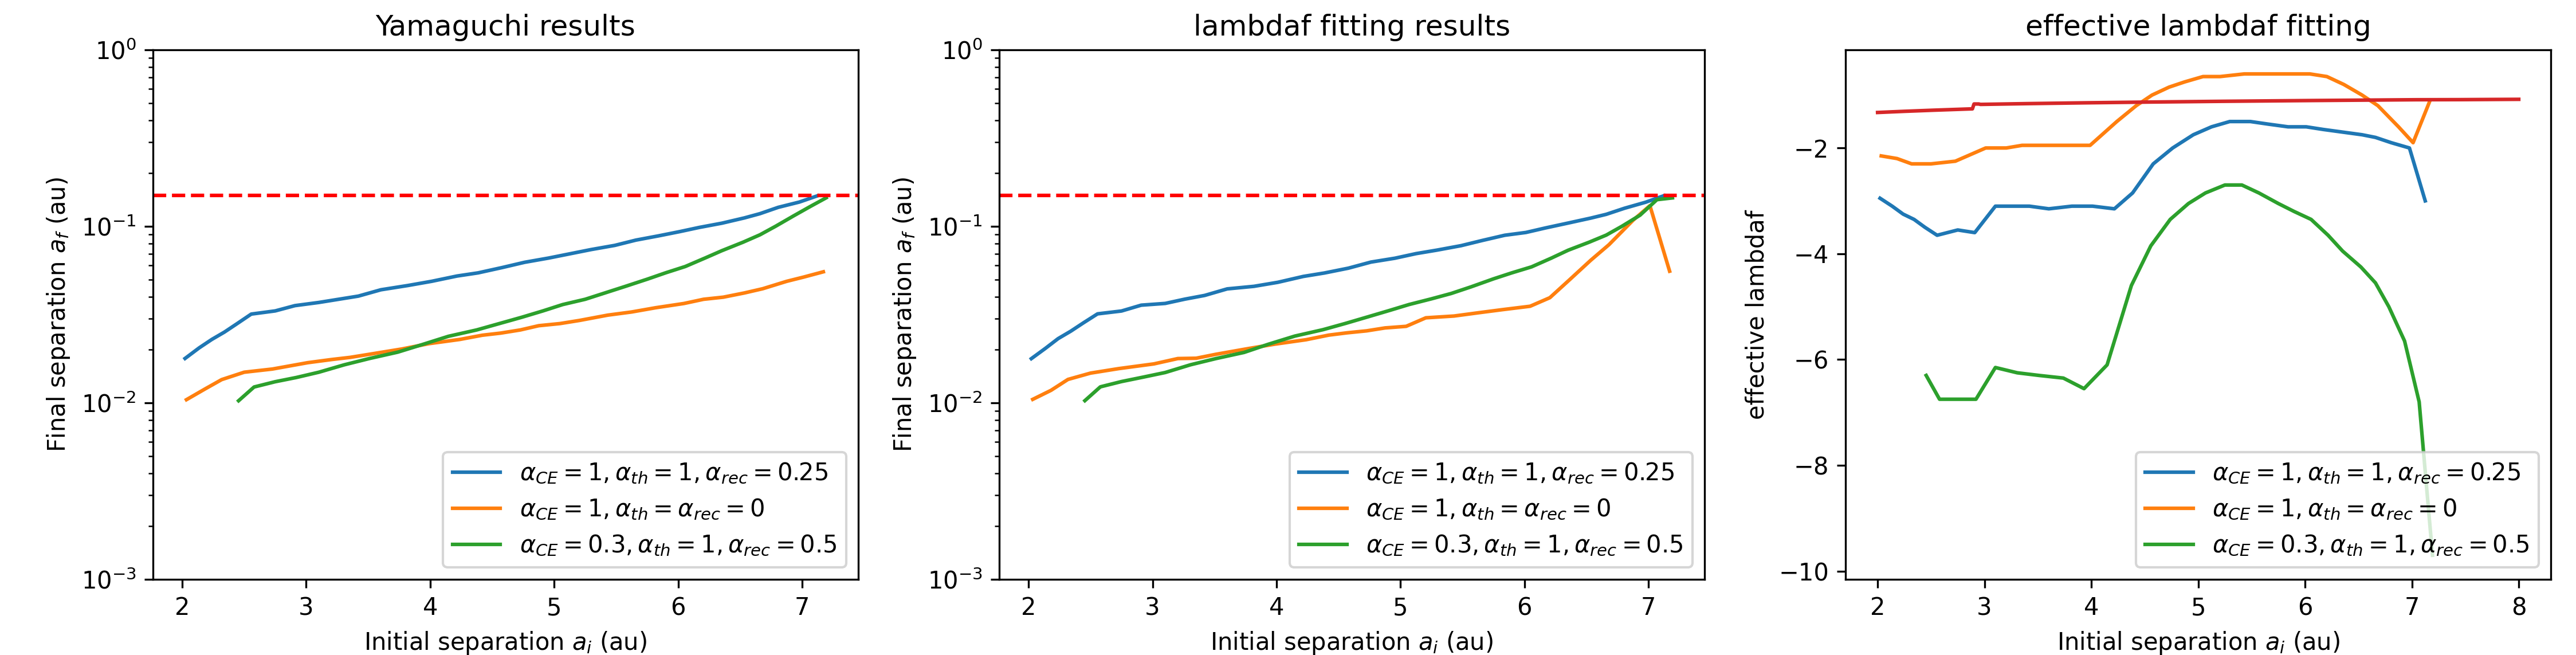
\includegraphics[width=0.9\linewidth]{7+1ebcmp.png}
	\caption{Same as Figure \ref{fit_cmp_hi}, but with a different energy budget — $\Ebind = \Egrav + \alphath \Eth + \alpharec \Erec$.}
	\label{fit_cmp_eb_hi}
\end{figure}

In Figure \ref{fit_cmp_eb_hi}, we present the same results for another energy budget of the CE process — $\Ebind = \Egrav + \alphath \Eth + \alpharec \Erec$.

\subsection{Low Mass Systems $(1.5 \Msun + 0.85 \Msun)$} \label{subsec:low}
In \cite{yamaguchi_lo}, the WD mass in the Gaia sample ranges from $0.5\Msun$ to $0.8\Msun$, which corresponds to progenitor mass of $1 \Msun$ to $3 \Msun$. The companions mass has a median of $0.85 \Msun$. MESA results for $1.5\Msun + 0.85\Msun$ systems is documented in \cite{yamaguchi_hi}. Hence, we consider a $1.5\Msun + 0.85\Msun$ evolution model in COSMIC and compare the results with those in \cite{yamaguchi_hi}.


\section{Stable Mass Transfer} \label{sec:stable}

\section{Population} \label{sec:population}


\bibliography{reference.bib}
\bibliographystyle{aasjournal}

\end{document}

